\documentclass[a4paper,11pt]{article}

\usepackage{mathtools}
\usepackage{amssymb}
\usepackage{hyperref}
\usepackage[cm]{fullpage}
\usepackage{fancyhdr}
\usepackage[ddmmyyyy]{datetime} 
\usepackage[]{graphicx}
\usepackage[ruled]{algorithm2e}
\usepackage{hhline}
\usepackage{listings}
\usepackage{enumitem}
\usepackage{cleveref}
\usepackage{todonotes}

%\renewcommand{\familydefault}{\sfdefault}

\graphicspath{{figures}}

% Settings for listings package
\definecolor{mygreen}{rgb}{0,0.6,0}
\definecolor{mygray}{rgb}{0.5,0.5,0.5}
\definecolor{mymauve}{rgb}{0.58,0,0.82}
\definecolor{altblue}{rgb}{0.0,0.6,1.0}
\definecolor{lstbg}{gray}{0.9}

\lstset{
  backgroundcolor=\color{lstbg},
  % choose the background color; you must add \usepackage{color} or \usepackage{xcolor}
  basicstyle=\footnotesize\ttfamily,
  % the size of the fonts that are used for the code
  breakatwhitespace=true,
  % sets if automatic breaks should only happen at whitespace
  breaklines=true,
  % sets automatic line breaking
  captionpos=b,
  % sets the caption-position to bottom
  commentstyle=\color{mygreen},
  % comment style
  deletekeywords={},
  % if you want to delete keywords from the given language
  escapeinside={\#*}{*},
  % if you want to add LaTeX within your code
  extendedchars=true,
  % lets you use non-ASCII characters; for 8-bits encodings only, does not work with UTF-8
  frame=single,
  % adds a frame around the code
  keepspaces=true,
  % keeps spaces in text, useful for keeping indentation of code (possibly needs columns=flexible)
  keywordstyle=\color{blue},
  % keyword style
  %language=c++,
  % the language of the code
  otherkeywords={},
  % if you want to add more keywords to the set
  numbers=left,
  % where to put the line-numbers; possible values are (none, left, right)
  numbersep=5pt,
  % how far the line-numbers are from the code
  numberstyle=\tiny\color{mygray},
  % the style that is used for the line-numbers
  rulecolor=\color{black},
  % if not set, the frame-color may be changed on line-breaks within not-black text (e.g. comments (green here))
  showspaces=false,
  % show spaces everywhere adding particular underscores; it overrides 'showstringspaces'
  showstringspaces=false,
  % underline spaces within strings only
  showtabs=false,
  % show tabs within strings adding particular underscores
  stepnumber=1,
  % the step between two line-numbers. If it's 1, each line will be numbered
  stringstyle=\color{mymauve},
  % string literal style
  tabsize=4,
  % sets default tabsize to 4 spaces
  title=\lstname
  % show the filename of files included with \lstinputlisting; also try caption instead of title
}

\hypersetup{
	colorlinks=true,
	allcolors=blue
}

\title{\textsc{Scalable and robust Firedrake deployment on ARCHER2 and beyond}\\
\Large ARCHER2-eCSE04-5}
\author{Jack Betteridge}
\date{30/4/2022}
% PI: Dr David A Ham (Imperial College) 

\pagestyle{fancy}
\setlength{\headheight}{15pt}
\setlength{\headsep}{5pt}
\lhead{ \fancyplain{}{} }
\rhead{ \fancyplain{}{Jack Betteridge} }
%\lhead[\footnotesize\nouppercase{\leftmark}]{}
%\rhead[]{\footnotesize\nouppercase{\rightmark}}

\renewcommand{\footrulewidth}{0.4pt}
\cfoot[-- \thepage\ --]{-- \thepage\ --}

\begin{document}
\maketitle

\begin{abstract}
	We summarise the different aspects of Firedrake deployment that we have improved for our HPC users and additional benefits for ARCHER2 users.
	\begin{enumerate}
	\item A Spack package has been created for Firedrake many of its dependencies as well as determining a suitable Spack configuration and package workflow for ARCHER2.
	\item Firedrake has been containerised for HPC resulting in a Singularity container suitable for use on ARCHER2.
	\item A fix has been provided to PETSc/petsc4py to reduce the occurrence of deadlock issues when running Firedrake scripts in parallel on HPC systems.
\end{enumerate}
\end{abstract}

%%%%%%%%%%%%%%%%%%%%%%%%%%%%%%%%%%%%%%%%%%%%%%%%%%
\section{Introduction}
\label{sec:intro}
%%%%%%%%%%%%%%%%%%%%%%%%%%%%%%%%%%%%%%%%%%%%%%%%%%
Firedrake is an automated system for the solution of partial differential equations using the finite element method (FEM) and sophisticated code generation.
The goal for this project was to make installing and running the Firedrake framework\cite{firedrakeweb,firedrakepaper}, and its many dependencies, simple and robust on any HPC platform, with a primary focus on ARCHER2.
We are confident in stating that this has been accomplished.
Whilst there is still maintenance and upkeep of the devised solutions we have largely achieved what we set out to accomplish in this eCSE.

\noindent Namely we have:
\begin{enumerate}[topsep=2pt, partopsep=0pt, itemsep=1pt, parsep=1pt]
    \item Developed a Spack package for Firedrake.
	\item Built a Singularity container for ARCHER2.
	\item Improved the robustness of PETSc's Python support.
\end{enumerate} 

We have reordered these accomplishments in what follows to highlight the revised importance compared to the initial proposal.
Namely that the development of a Spack package for Firedrake was a more complicated undertaking than originally thought, but additionally this work may have a larger impact for a wider range of ARCHER2 users.


%%%%%%%%%%%%%%%%%%%%%%%%%%%%%%%%%%%%%%%%%%%%%%%%%%
\section{Firedrake Spack Package}
\label{sec:spack}
%%%%%%%%%%%%%%%%%%%%%%%%%%%%%%%%%%%%%%%%%%%%%%%%%%
Spack\cite{spackweb,spackpaper} is a popular choice of package manager for HPC users to install packages with complex dependencies.
Firedrake previously did not support installation via Sapck, but it is one of the few package managers capable of delivering the fine grained control over build dependencies and is designed with HPC in mind.
Furthermore, Spack can take advantage of any dependencies already available on a given system, either available through the OS or through the module system.

%%%%%%%%%%%%%%%%%%%%%%%%%%%%%%%%%%%%%%%%%%%%%%%%%%
\subsection{Previous situation}
\label{ssec:prev}
%%%%%%%%%%%%%%%%%%%%%%%%%%%%%%%%%%%%%%%%%%%%%%%%%%
Prior to this work the installation path was the same on a HPC system as it would be on any other computer, namely use the Firedrake install script (\cref{lst:firedrake-install}).
\begin{lstlisting}[float,caption={Firedrake install script install commands},label={lst:firedrake-install}]
curl -O https://raw.githubusercontent.com/firedrakeproject/firedrake/master/scripts/firedrake-install
python3 firedrake-install
\end{lstlisting}
The \verb`firedrake-install` command is a custom written Python script which can take numerous configuration arguments suitable for building Firedrake to the exact user specification.

Command line arguments can be used to specify the MPI distribution, an existing PETSc build if the user didn't want Firedrake to build its own, which BLAS/LAPACK libraries to link against and any other additional packages the user may want to install.
Much of the work done by this install script was to overcome limitations in each dependency's own build system.
It is important for Firedrake that everything is built using the same MPI distribution, if the wrong distribution gets initialised by a package, PETSc will not be able to start.
For instance, if \verb`mpi4py` is built against OpenMPI and PETSc uses MPICH, the installation is broken.
This is quite a common situation for other projects, but for Firedrake things are further complicated by dependencies in Python packages.
For instance, PETSc and Numpy must both be linked against the same BLAS/LAPACK libraries, to prevent a FORTRAN ABI mismatch.
If PETSc builds against a system install of NETLIB BLAS/LAPACK and Numpy uses the OpenBLAS bundled inside a pre-built wheel, again the installation is broken.

Many special configuration cases have been coded into the \verb`firedrake-install` script to ensure that, on as many systems that we know about, the user is left with a working Firedrake installation.
The issue on HPC is when installation fails, users may be forced to rewrite parts on the installation script for the system they are on in order to get installation to succeed.
For the end user the completed installation on their system is a Python virtual environment, which is self contained as much as possible.
This is the desktop user experience that we aim to recreate with the Spack package manager for HPC users.

\begin{figure}[htp]
	\centering
	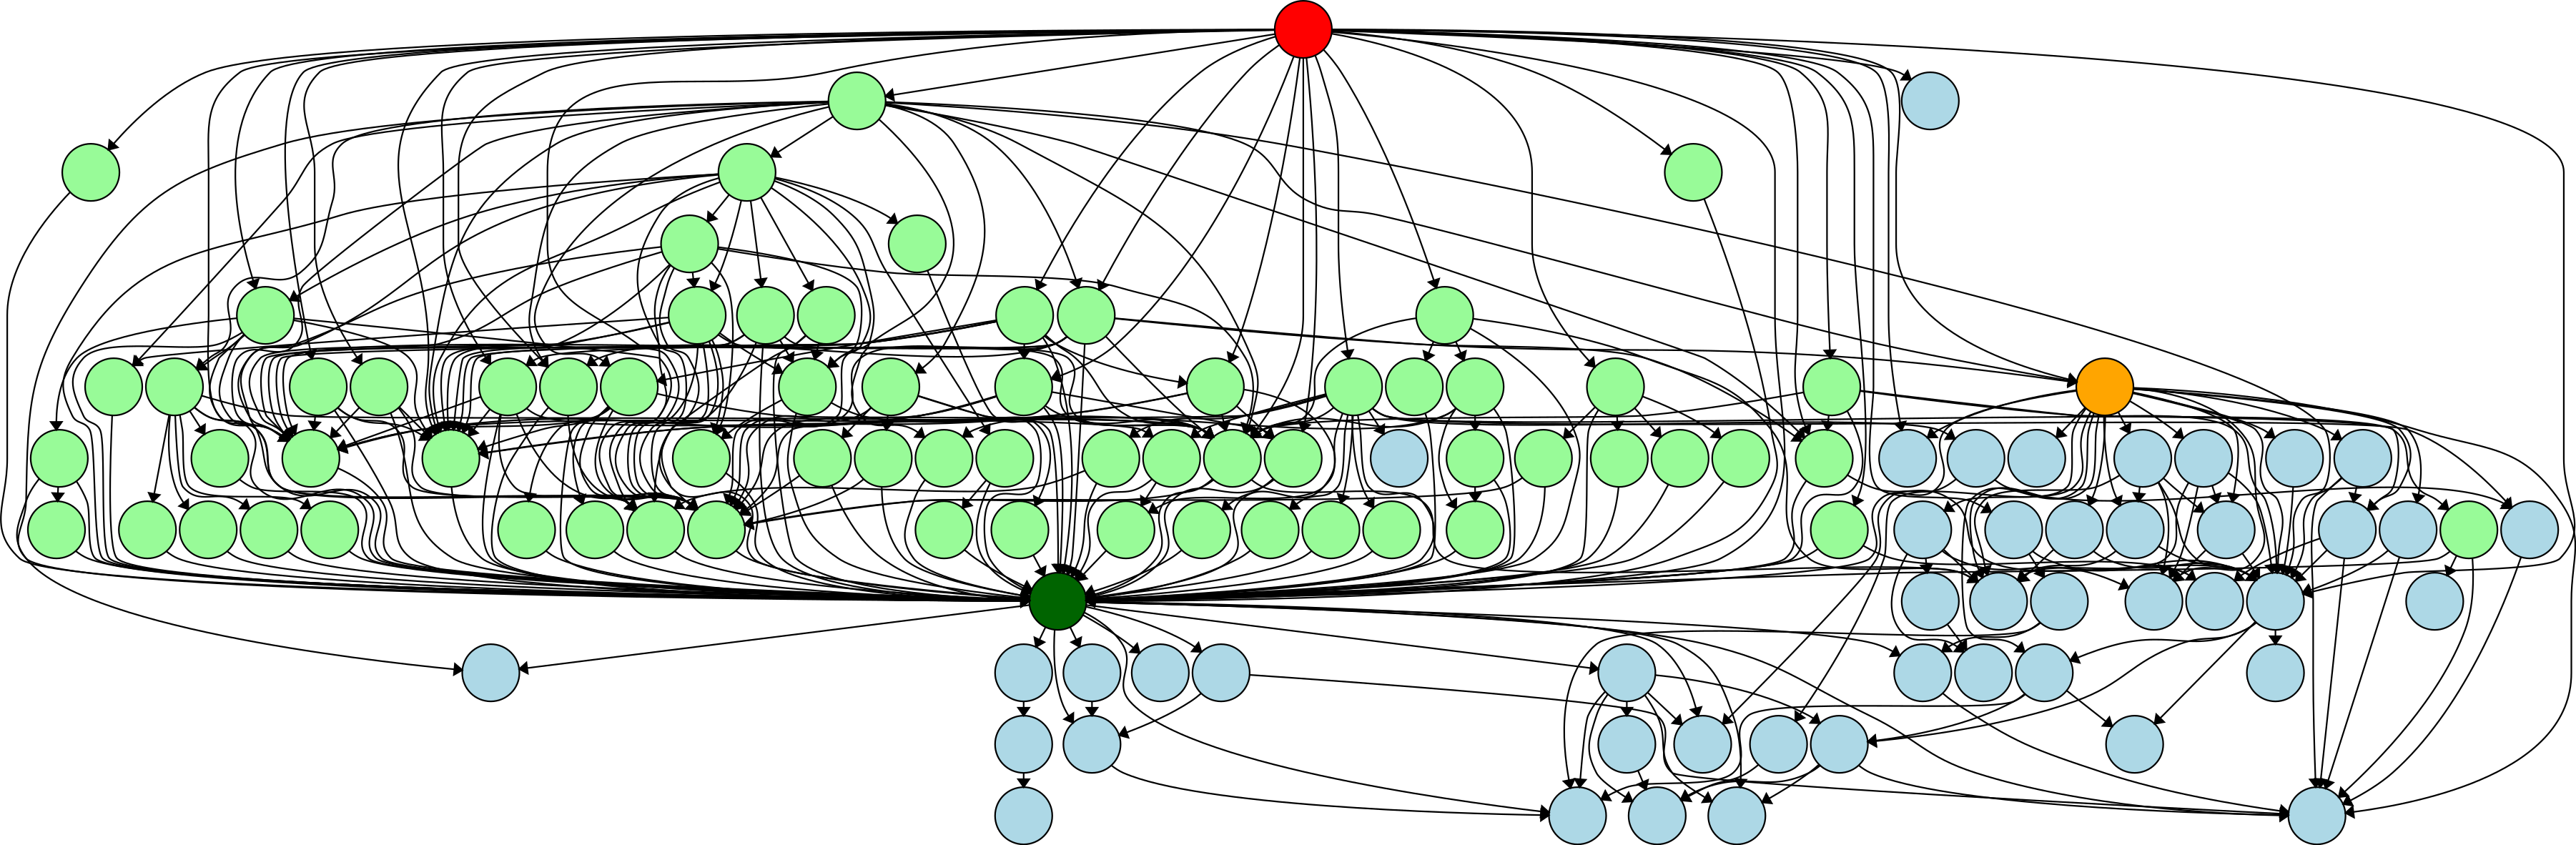
\includegraphics[width=\textwidth]{firedrake_deps.png}
	\caption{A directed graph showing the complexity of Firedrake's dependencies. Firedrake is highlighted at the top in red, Python as dark green and Python packages as light green. The orange circle is PETSc and all remaining pale blue circles are compiled dependencies. Generated by the command:\\ \texttt{spack graph -d py-firedrake \%gcc \^{}mpich \^{}openblas \textgreater{} py-firedrake.dot}}
	\label{fig:fddeps}
\end{figure}

%%%%%%%%%%%%%%%%%%%%%%%%%%%%%%%%%%%%%%%%%%%%%%%%%%
\subsection{Aims}
\label{ssec:spack_aims}
%%%%%%%%%%%%%%%%%%%%%%%%%%%%%%%%%%%%%%%%%%%%%%%%%%
From the outset we wanted any alternative installation to satisfy the following criteria:
\begin{enumerate}[topsep=2pt, partopsep=0pt, itemsep=1pt, parsep=1pt]
	\item To produce a working Firedrake installation on HPC machines.
	\item To have the same (or as similar as possible) functionality to a regular script based Firedrake installation.
	\item The new installation should require as little manual intervention as possible and should not require editing installation scripts or packages to succeed.
	\item Fit entirely into the chosen (Spack) framework. That is not to require additional functionality that isn't present in the existing framework.
	\item To make the installation more extensible and better compatible with external and alternative package providers, as are often present on HPC.
\end{enumerate}

%%%%%%%%%%%%%%%%%%%%%%%%%%%%%%%%%%%%%%%%%%%%%%%%%%
\subsection{Spack}
\label{ssec:spack}
%%%%%%%%%%%%%%%%%%%%%%%%%%%%%%%%%%%%%%%%%%%%%%%%%%
Spack was chosen as the build framework due to its explicit support for HPC and ease of installation for a HPC user, rather than administrator.
Spack already supports building many of Firedrake's dependencies, reducing the burden of maintenance for Firedrake developers.
There is also a concerted effort in the long term maintenance of Spack, many of the US national laboratories are now using Spack and software sustainability groups such as xSDK\cite{xSDK1,xSDK2} require packages to be Spack installable.
However, one criticism we have of the Spack package manager is the amount of work for a new user to learn and configure the tool.
We outline configuration here and have detailed instructions available online\cite{?}.

Before building Firedrake, Spack needs to be installed and configured to run on on ARCHER2.
Spack can be installed on any UNIX or UNIX like system, but special care must be taken on a HPC facility to ensure functionality with the rest of the system packages.

The ``installation'' of Spack is straightforward, it requires cloning the Spack git repository and calling an activation script.
Importantly, if there is no system installation of Spack, these steps can be performed easily as a HPC user without the need for administrative privileges.
Spack even supports ``chaining'' installations, where one instance of Spack can use the packages from another instance.
This will initially be very useful to us, as package updates that we have contributed are not yet in a versioned Spack release and many HPC systems will not update system modules unless there is a pressing reason to do so.

It's essential that a working Python interpreter is loaded as Spack is a Python program, the OS Python is often not sufficient as it is often out of date and missing key internal components which prevent Spack from working correctly.
It is our recommendation to load a Python module (such as \verb`cray-python` on ARCHER2) if it is available before calling the spack activation script.
After the activation step any Spack command can be invoked at the command line and users can start installing packages.

However, it is valuable to spend time configuring Spack for the HPC being used system.

%%%%%%%%%%%%%%%%%%%%%%%%%%%%%%%%%%%%%%%%%%%%%%%%%%
\subsection{Setup}
\label{ssec:setup}
%%%%%%%%%%%%%%%%%%%%%%%%%%%%%%%%%%%%%%%%%%%%%%%%%%
Without any external configuration Spack uses whichever C, C++ and FORTRAN compilers are available on the path and will not use any system packages, instead it will bootstrap its own build system.
While useful for systems with no package manager, or minimalist OS's, this is not ideal for HPC.
On a supercomputer we wish to make use of specific optimised compilers, MPI distributions that take advantage of the interconnect hardware and libraries optimised for the architecture.
Spack allows users to utilise this software, usually available as modules, through extensive configuration options.

The file
\footnote{\texttt{\$SPACK\_USER\_CONFIG} if not explicitly set will default to \texttt{\~{}/.spack}. This may cause issues if you attempt to build packages on a computer node of ARCHER2 as the default home directory is not mounted.}
\verb`$SPACK_USER_CONFIG/<system>/compilers.yaml` is read by Spack to determine what additional compilers are available on the system.
On ARCHER2 we initially populated this file by running the command:
\begin{lstlisting}[numbers=none]
spack compiler find	
\end{lstlisting}
Spack does a reasonable job of populating this file with the correct compiler specs as well as appropriate compiler flags and even configures the correct modules to load to use the compilers.
It is still worth checking this file carefully, as any error here may require all packages built with that compiler to be rebuilt.

A similar trick can be used to populate \verb`$SPACK_USER_CONFIG/packages.yaml`, which is read by spack to determine additional packages that can be used.
However,
\begin{lstlisting}[numbers=none]
spack external find	
\end{lstlisting}
only picks up build dependencies (tools like Bison, m4, git and tar), not the modules available on the system.
Care must be taken to add \verb`cray-mpich` as the MPI provider along with a suitable spec line, additional modules to load, the prefix path and tag the package as not buildable by Spack.
The same procedure must be done for the BLAS and LAPACK provider (\verb`cray-libsci`) and the Python module, if they are desired as build dependencies, otherwise Spack will build its own copy.

Setting this up may be daunting for a user, but is possible to have a centrally installed instance of Spack or a centrally managed global Spack configuration (one that is overridden by the user's configuration, if desired).
Once build configurations have been finalised the Spack settings documented on the Firedrake wiki\cite{firedrakewiki} could be used as the ARCHER2 global configuration.
Up until this point nothing has been Firedrake specific and is a useful introduction for anybody starting out using Spack on ARCHER2.

The \href{https://github.com/firedrakeproject/firedrake-spack}{Firedrake spack repository} currently holds all of the additional packages currently required to build Firedrake.
This repo works in conjunction with the Spack's \verb`builtin` repo, offering additional packages and modifications of existing packages.
\Cref{ssec:changes} contains some examples.

Users can add the Firedrake Spack repo by cloning the remote repository and adding the repo to Spack's configuration:
\begin{lstlisting}
git clone https://github.com/firedrakeproject/firedrake-spack.git
spack repo add firedrake-spack
\end{lstlisting}

In order to isolate the packages for the Firedrake installation in the same way that Python's venv does, the Spack installation uses Spack environments.
This gives a very similar end user experience for anyone who has previously installed Firedrake using the install script.
It also allows for packages to be added in the environment, with a prefix under the environment directory, giving a developer the same freedom to make changes to packages, whilst keeping all the core dependencies in one place.

The environment is created, activated and populated with the core packaged by executing:
\begin{lstlisting}
spack env create -d ./firedrake
spack env activate -p ./firedrake

spack develop py-firedrake@develop
spack develop py-pyop2@develop
...
\end{lstlisting}

Currently the core packages are added one at a time, and a typical Spack Firedrake environment consits of:
\begin{lstlisting}
$ ls firedrake/
chaco        petsc   py-codepy py-fiat  py-firedrake py-islpy py-petsc4py  py-pyop2 py-ufl
libsupermesh py-cgen py-coffee py-finat py-genpy     py-loopy py-pyadjoint py-tsfc
\end{lstlisting}
At this point both the Spack build system and the Firedrake environment are configured and Firedrake can be installed.


%%%%%%%%%%%%%%%%%%%%%%%%%%%%%%%%%%%%%%%%%%%%%%%%%%
\subsection{Upstream changes}
\label{ssec:changes}
%%%%%%%%%%%%%%%%%%%%%%%%%%%%%%%%%%%%%%%%%%%%%%%%%%
PETSc is one of the key dependencies of Firedrake and it is essential for core functionality that PETSc builds correctly, with all of its own dependencies and links against all libraries necessary for Firedrake to function.
For stability, Firedrake maintains its own fork of PETSc tracking a few commits behind PETSc main, so it is necessary to create a modified package maintained in the Firedrake Spack repo that points to this fork.
Changing the location of the source code could never be incorporated into the builtin Spack PETSc package, which necessitated its duplication in our own repository.
A key contribution from this eCSE was the modification of the builtin PETSc package, to allow for inheritance and modification enabling the package to be subclassed without having to re-implement the install logic.
This now allows other projects to create alternative PETSc installs using the Spack builtin as a parent class.
Chaco, Eigen, NetCDF and parallel NetCDF have been included as options in the Firedrake PETSc Spack package, since these libraries need to be linked against for a working installation.

Chaco, a mesh partitioner developed at Sandia, is an upstream package that has not seen active development for many years and did not previously have a Spack package\footnote{or at least didn't when the project started}, so this is also included in the Firedrake package repo.

In \cref{ssec:prev} it was mentioned that Numpy (and Scipy) need to be linked against the same BLAS and LAPACK providers as PETSc to allow both to be imported in Python.
This eCSE expanded the number of different BLAS/LAPACK implementations that Numpy could build against as options in Spack.
This enables compatibility with both the AMD Optimizing CPU Libraries and Cray scientific libraries available on ARCHER2.
Additional logic has also been added to the Scipy package to ensure that it too is built with the same BLAS/LAPACK as Numpy.
These changes have been merged into the development branch of Spack for the benefit of all Spack users.

To allow for the use of different compilers in Spack modifications had to be made to the PyOP2 package, which handles the compilation stage of the code generation within Firedrake.
Refactoring allows end users to customise the compiler and compiler flags used with PyOP2 by creating new Python compiler classes, as well as allowing the default compiler classes to be overridden by environment variables.
These environment variables can be automatically set when Spack loads the Firedrake environment.
Now by default PyOP2 will use the same compiler that Spack used to build the rest of the Firedrake dependency tree.

Python packages within a Firedrake environment are installed in ``developer mode'', which allows for the source code in the cloned git repository to be used as if it were installed to Python's site-packages directory.
This behaviour is not natively supported by Spack, but we have developed an \verb`EditablePythonPackage` class in the \verb`editable_install` package, which allows core dependencies to be installed in developer mode.

In addition to these changes the following is an exhaustive list of new or modified Spack packages that were created for this work:
\begin{lstlisting}
$ ls firedrake-spack/packages
chaco             py-cgen     py-firedrake     py-icepack  py-petsc4py   py-pytools
editable_install  py-codepy   py-folium        py-irksome  py-pulp       py-thetis
libspatialindex   py-coffee   py-genpy         py-islpy    py-pyadjoint  py-tsfc
libsupermesh      py-femlium  py-geojson       py-loopy    py-pygmsh     py-ufl
petsc             py-fiat     py-gmsh-interop  py-meshio   py-pymbolic   py-uptide
py-branca         py-finat    py-gusto         py-meshpy   py-pyop2      py-vtk
\end{lstlisting}
These will be offered to the maintainers of each project for their inclusion into Spack's builtin repository to ensure better package maintenance.


%%%%%%%%%%%%%%%%%%%%%%%%%%%%%%%%%%%%%%%%%%%%%%%%%%
\subsection{The \texttt{py-firedrake} package}
\label{ssec:py-firedrake}
%%%%%%%%%%%%%%%%%%%%%%%%%%%%%%%%%%%%%%%%%%%%%%%%%%
The Spack package for Firedrake supports all the same functionality as the previous Firedrake install script including installing additional packages, specifying the MPI to use for dependencies and allowing foll customisation of PETSc build options.
All this functionality fits into the Spack spec ``language'' for specifying versions and options for packages.
For instance, if running on a local machine where the user wants Spack to build all dependencies, Firedrake can be configured using the GCC compiler, MPICH and OpenBLAS using the command:
\begin{lstlisting}
spack add py-firedrake@develop %gcc ^mpich ^openblas
spack install
\end{lstlisting}

On ARCHER2, Firedrake can be configured with gcc, Cray Python, the Cray Scientific Libraries and Cray MPICH (if have been added to the list of external packages) using the command in \cref{lst:spackarcher2}.
\begin{lstlisting}[float,caption={Spack configuration for ARCHER2 using GCC, Cray Python, Cray MPICH and Cray scientific libraries},label={lst:spackarcher2}]
spack add py-firedrake@develop \
    %gcc@10.2.0 \
    ^python@3.9.4.1 \
    ^cray-mpich@8.1.9%gcc@10.2.0 \
    ^cray-libsci@21.04.1.1
spack install
\end{lstlisting}
Furthermore the Firedrake Spack package includes additional functionality that cannot be added to script.
One additional feature is using system packages and more importantly system modules as part of a Firedrake build.
Another is the ability to specify the compiler for the whole toolchain.
When the Firedrake installation script is used packages are not all guaranteed to use the same compiler.
Changes to the PyOP2 package, as noted in \cref{ssec:changes}, make it possible for Spack to set the default compiler for PyOP2 to use for code generation when the Spack environment is activated.

Extensive instructions are currently held in a working document (currently available on \href{https://hackmd.io/Sg3fYXuCTl61d_LAg4QnMw}{hackmd}), which will be added to the \href{https://github.com/firedrakeproject/firedrake/wiki}{Firedrake wiki}\cite{firedrakewiki} and we hope to contribute these instructions and instructions for using Spack to the \href{https://docs.archer2.ac.uk/}{ARCHER2 documentation}\cite{archer2docs} site.

To test the portability of the Spack installer, it has also been successfully tested on different platforms:
\begin{itemize}[topsep=2pt, partopsep=0pt, itemsep=1pt, parsep=1pt]
	\item Tier 2 HPC facility Isambard (XCI ThunderX2)
	\item HPC facilities at Imperial College
	\item HPC facilities at UCL
	\item Numerous end users personal machines, comprising different architectures
\end{itemize} 
An additional configuration is being developed that utilises the NVidia compilers, to maximise performance on ARM hardware and will no doubt be useful in the future work porting Firedrake to GPUs as part of code generation's road to exascale.

We would like to acknowledge the help of Connor Ward who helped with the initial generation of many of the Spack packages used as part of this work.


%%%%%%%%%%%%%%%%%%%%%%%%%%%%%%%%%%%%%%%%%%%%%%%%%%
\section{Singularity}
\label{sec:singularity}
%%%%%%%%%%%%%%%%%%%%%%%%%%%%%%%%%%%%%%%%%%%%%%%%%%
In order to support containerisation on ARCHER2, we need to create a Singularity image.
For several years the Firedrake developers have been building several working Docker containers with many different flavours of Firedrake installation.
These include:
\begin{itemize}[topsep=2pt, partopsep=0pt, itemsep=1pt, parsep=1pt]
	\item \verb`firedrake-env` - The build environment, Ubuntu 20.04 with all required system packages, but without Firedrake.
	\item \verb`firedrake-vanilla` - Firedrake with no additional packages or associated applications, which forms the base image for the remaining flavours.
	\item \verb`firedrake` - Firedrake with some additional Firedrake applications bundled (Gusto, Thetis, Icepack, etc...).
	\item \verb`firedrake-complex` - The same as \verb`firedrake`, but with support for complex numbers.
	\item \verb`firedrake-notebooks` - A container with both Firedrake and Jupyter notebooks installed, for running tutorials.
\end{itemize}    
By using CI automation these Docker images can be kept up to date with every successful build.

Unfortunately, Docker is not a suitable container format for running on HPC as it allows for privilege escalation.
The Apptainer/Singularity\footnote{Singularity used to be the name of both a closed source and open source project. These projects have diverged and the open source project is now called Apptainer and the closed source project is called Singularity. The executable is still called \texttt{singularity} in both cases, so we use this name in the report.} 
project aims to perform the same role as Docker, but without the same security vulnerability so that images may be used on any HPC facility that supports containers.

In order to maintain a single source for the Firedrake container our work has focused on modifying the Docker container so that it may be converted to a usable Singularity container.
Singularity allows images to be converted using the command in \cref{lst:singularity-docker} (using the \verb`firedrake-vanilla` container as an example throughout).
\begin{lstlisting}[numbers=none,float,caption={One step (pull and) conversion from Docker image format to Singulrity image format},label={lst:singularity-docker}]
singularity pull firedrake-vanilla.sif docker://firedrakeproject/firedrake-vanilla
\end{lstlisting}
However, this does not work for Firedrake images, since the \verb`firedrake` virtual environment is built in the \verb`$HOME` directory.

We have found that it is possible to convert the Docker image to an Singularity image in a two step procedure using a sandbox environment to prevent changes to the \verb`$HOME` environment within the container:
\begin{lstlisting}[caption={Two step procedure 1. (pull and) build with sandbox from Dockerhub, 2. Build Singulrity image format},label={lst:singularity-docker2}]
singularity build --sandbox ./firedrake-vanilla docker://firedrakeproject/firedrake-vanilla
singularity build firedrake-vanilla.sif ./firedrake-vanilla
\end{lstlisting}
Both of these commands can be executed without administrative privileges, so are still suitable for end users on ARCHER2.
This saves both having to host the Singularity image or the user having to upload the large image from a personal machine.

The Docker images have been updated to include some additional system packages, such as the OpenFabric library, to enable the resultant Singularity image to be compatible with ARCHER2.
Any of the Firedrake Docker images listed above can be converted using \cref{lst:singularity-docker2}, not just \verb`firedrake-vanilla`.

When configuring the image for running under MPI, there is a choice of hybrid or bind model.
In the bind model the container has no MPI installation and instead the host system MPI is mounted within the container (AKA binding) and all packages in the image are linked against this MPI.
Such a model is not suitable for Firedrake as it would require too many changes.
We wouldn't be able to start from the Docker image, as these require an MPI installation to work, and this would necessitate building the Singularity image from scratch.
Building from scratch is also not really an option, since this process requires ARCHER2 to use the Cray's MPICH would need to be performed with administrative permissions (which we cannot have).

Instead we use the hybrid model, which is recommended in the ARCHER2 container course, involves using the MPI executable from the host.
The application in the container is linked against and uses the MPI installation within the container which has the ability to communicate with the MPI daemon process running on the host system.

With the image built we can begin running applications in the Singularity container.
Following ARCHER2 documentation\cite{archer2docs}, we use \verb` cray-mpich-abi` in place of \verb`cray-mpich` and set the environment variables \verb`SINGULARITYENV_LD_LIBRARY_PATH` and \verb`SINGULARITY_BIND` appropriately.
This enables additional Cray libraries and hardware specific device libraries to be found by executables inside the container.
%\begin{lstlisting}
%export SINGULARITYENV_LD_LIBRARY_PATH=
%    /opt/cray/pe/mpich/8.1.9/ofi/gnu/9.1/lib-abi-mpich:
%    /opt/cray/pe/pmi/6.0.10/lib:/opt/cray/libfabric/1.11.0.4.71/lib64:
%    /usr/lib64/host:/usr/lib/x86_64-linux-gnu/libibverbs:
%    /.singularity.d/libs:/opt/cray/pe/gcc-libs
%export SINGULARITY_BIND=
%    "/opt/cray,/usr/lib64/libibverbs.so.1,
%    /usr/lib64/librdmacm.so.1,/usr/lib64/libnl-3.so.200,
%    /usr/lib64/libnl-route-3.so.200,
%    /usr/lib64/libpals.so.0,
%    /var/spool/slurmd/mpi_cray_shasta,
%    /usr/lib64/libibverbs/libmlx5-rdmav25.so,
%    /etc/libibverbs.d,
%    /opt/gcc"
%\end{lstlisting}

Additional environment variables can be set within the container be prepending them with \verb`SINGULARITYENV_`.
We use this to control the location of the various cache directories, to ensure they are writable, and to locate the correct compilers inside the container:
\begin{lstlisting}
export SINGULARITYENV_OMP_NUM_THREADS=1
export SINGULARITYENV_PYOP2_CACHE_DIR=/tmp/$USER/pyop2
export SINGULARITYENV_PYOP2_CC=/home/firedrake/firedrake/bin/mpicc
export SINGULARITYENV_PYOP2_CXX=/home/firedrake/firedrake/bin/mpicxx
export SINGULARITYENV_FIREDRAKE_TSFC_KERNEL_CACHE_DIR=/tmp/$USER/tsfc
\end{lstlisting}

Finally, when running Singularity additional steps must be taken to ensure that the Firedrake script is visible inside the container.
By default Singularity will bind (mount within the container) various directories, including the host \verb`$HOME` directory, and execute programs as the host system user (not the container user) using the mounted \verb`$HOME` directory inside the container as the working  directory.
Care must therefore be taken to additionally bind any directories where scripts reside and where results will be saved, since an ARCHER2 user's \verb`$HOME` directory is not mounted on compute nodes.

In the following example the \verb`--home` argument binds the current working directory (\verb`$PWD`) as the \verb`$HOME` directory for the container, overriding the default behaviour.
Additionally, the current working directory is bound to the mount point \verb`/home/firedrake/work`, using \verb`--bind` so that scripts can be found when running in the container and results can be saved.
The choice of these mount locations can be changed by the user to the location of their scripts, results directories and possibly as "home space" located under the \verb`/work` directory as needed.
Finally, the Python installed in the \verb`firedrake` user's home directory is used to execute a script in the bound directory \verb`/home/firedrake/work/`.

\begin{lstlisting}
srun --ntasks-per-node 128  \
    singularity run --bind $PWD:/home/firedrake/work --home $PWD firedrake-vanilla.sif \
        /home/firedrake/firedrake/bin/python \
            /home/firedrake/work/myScript.py
\end{lstlisting}
Whilst there are a lot of options here, it gives the end user complete control over what locations on the ARCHER2 system are available for reading and writing by the container.
Furthermore, using a container involves no installation for the user, just configuration.

!!!Performance comparison!!!


%%%%%%%%%%%%%%%%%%%%%%%%%%%%%%%%%%%%%%%%%%%%%%%%%%
\section{Clean up of parallel objects in PETSc}
\label{sec:other}
%%%%%%%%%%%%%%%%%%%%%%%%%%%%%%%%%%%%%%%%%%%%%%%%%%
Prior to the start of this eCSE we observed an issue when running Firedrake in parallel.
When running on ARCHER2 (and other HPC facilities) jobs would randomly hang, with no apparent cause.
On repeating the same job, it may then complete with no hang.
Fixing the issue involved adding additional functionality to PETSc, the Portable, Extensible Toolkit for Scientific Computation\cite{petsc}.

The source of this issue was determined to be Python's garbage collector.
Specifically when running under MPI, Python objects created using petsc4py are allowed to be cleaned up by the cyclic garbage collector, causing simulations to deadlock.
This happens because petsc4py objects are distributed across ranks and as such require synchronised destructon, but Python is not MPI aware and calls the garbage collector at different times on different ranks.

Whilst ARCHER2 isn't the first platform on which this problem has been observed, the combination of high core count per job and large number of Python objects created in certain algorithms meant a high prevalence of the issue during our previous simulations.
The problem is very relevant to this eCSE as it affects both the scalability and robustness of Firedrake.
Since the issue only occurs in parallel, and the more MPI ranks used the higher the chance one Python instance calls the garbage collector out of turn means that any HPC platform is vulnerable to this issue.
Furthermore, it can result extreme costs for HPC users as deadlocks do not terminate jobscripts.
Instead it will waste all the Compute Units (CUs) assigned to a particular job and waste a lot of an end users time trying to track down the cause of the deadlock.

The solution we present performs the job of the cyclic garbage collector safely for Single Program Multiple Data (SPMD) programs.
This is done in three stages:
\begin{enumerate}
	\item \label{item:create}\textbf{Creation} (Synchronous)
	At object instantiation the current number of objects associated with the current communicator is attained and incremented.
	This creation index is associated with that object for its lifetime.
	\item \label{item:destroy}\textbf{Delayed destruction}(Non-synchronous)
	At object destruction a reference to the underlying struct is held and added to a garbage hashmap using the creation index as the key.
	The memory is not yet freed as a reference to the struct persists.
	Since this step is non-synchronous it can safely be called at any time by Python's garbage collector.
	\item \label{item:cleanup}\textbf{Cleanup}(Synchronous)
	A cleanup routine is periodically called on all ranks within the communicator to deallocate the memory occupied by the structs present in the garbage hashmap 
	\begin{itemize}[topsep=0pt, partopsep=0pt, itemsep=1pt, parsep=1pt]
	\item \emph{that have been destroyed on all ranks,}
	\item \emph{and in ascending creation index order}.
    \end{itemize}
    \Cref{alg:cleanup} outlines the procedure used for this step.
\end{enumerate}

\begin{algorithm}[htp]
	\SetKwBlock{Function}{cleanup(comm)}{return}
	\Function(){
		garbage = getGarbage(comm)\\
		sorted\_keys = sort(garbage.keys())\\
		intersection = gatherIntersect(comm, sorted\_keys)\\
		\For{\emph{key in intersection}}{
			object = garbage.get(key)\\
			object.collectiveDestroy()\\
			garbage.remove(key)
		}
	}
	\caption[]{Parallel garbage collection function}
	\label{alg:cleanup}
\end{algorithm}

\begin{figure}[htp]
	\centering
	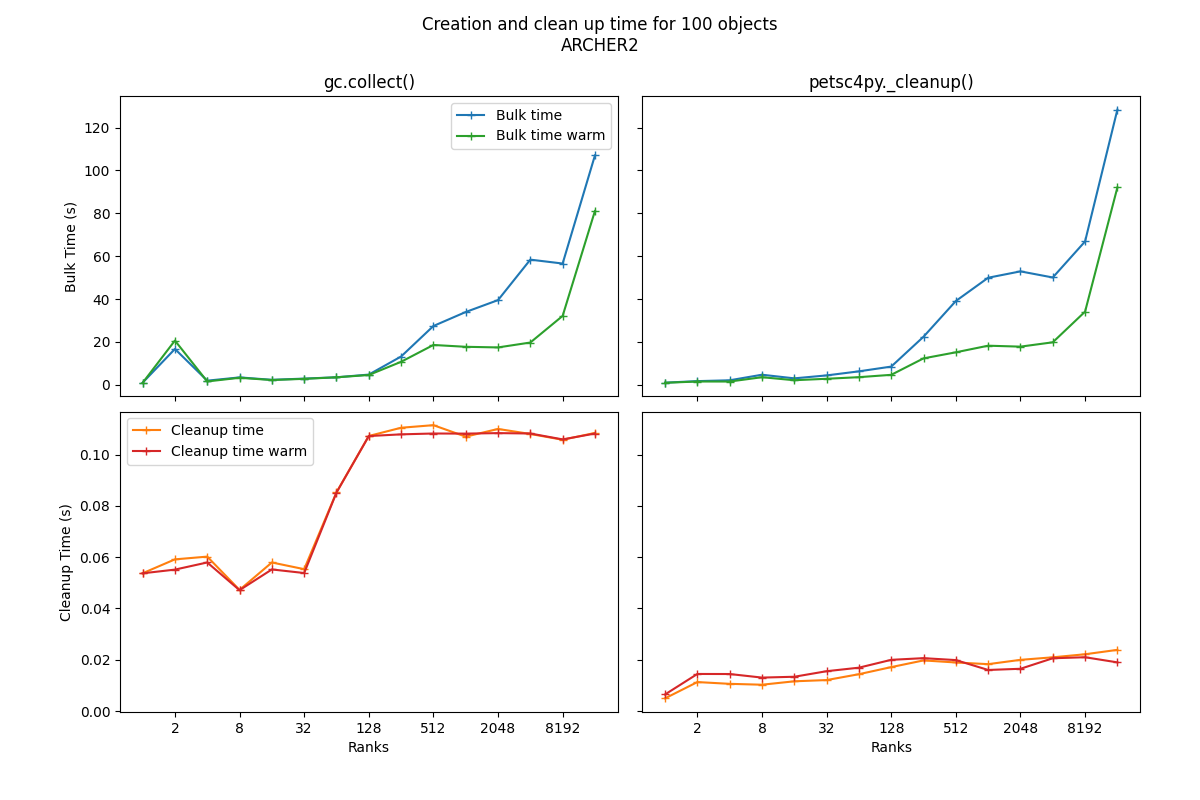
\includegraphics[width=\textwidth]{D100BS128B_222.png}
	\vspace{-1em}
	\caption{Performance comparison of bulk (object creation time), both top, and cleanup time, both bottom, for simulations using the broken object cleanup procedure, both left, compared to the newly implemented parallel safe cleanup, both right. Runs were performed with both cold and warm caches.}
	\label{fig:perf_comp}
\end{figure}

These changes are completely transparent to the end user, when this fix gets merged into PETSc no changes will need to be made to existing codes.
At this point Firedrake scripts will no longer hang in parallel due to the garbage collection issue, preventing wasted resources when running jobs.
By merging this fix into upstream PETSc, it will benefit all petsc4py users, not just Firedrake users.

Preliminary results indicate that the fix will have little impact on the performance of code after the fix is merged.
\Cref{fig:perf_comp} shows the time to create 100 distributed objects (bulk time) and the time taken to clean up the memory from the objects when they have been destroyed (cleanup time).
These times are presented for two different methods, the two plots on the left are indicative of the performance before the fix and experiments are prone to hang, the plots on the right show the performance with the fix implemented.
Two lines are shown on each plot, the time to create/destroy the objects with a cold cache (simply labelled `time') and time to create/destroy the objects on a second run with populated Python caches (labelled `time warm').

The techniques used in this improvement to PETSc/petsc4py will be explored in an upcoming publication.


%%%%%%%%%%%%%%%%%%%%%%%%%%%%%%%%%%%%%%%%%%%%%%%%%%
\appendix
\section{Appendix}
\label{sec:app}
%%%%%%%%%%%%%%%%%%%%%%%%%%%%%%%%%%%%%%%%%%%%%%%%%%
\subsection{Spindle}
\label{ssec:spindle}
%%%%%%%%%%%%%%%%%%%%%%%%%%%%%%%%%%%%%%%%%%%%%%%%%%


%%%%%%%%%%%%%%%%%%%%%%%%%%%%%%%%%%%%%%%%%%%%%%%%%%
\subsection{Tarballing}
\label{ssec:tarball}
%%%%%%%%%%%%%%%%%%%%%%%%%%%%%%%%%%%%%%%%%%%%%%%%%%

\bibliographystyle{abbrv}
\bibliography{references}


\end{document}